\documentclass{article}
\usepackage[utf8]{inputenc}
\usepackage{graphicx}
\usepackage{xcolor}
\usepackage{listings}

\title{Trabalho Final PDI\\
	Utilização de técnicas de detecção de faces em imagens de baixa resolução\\}
\author{\\Departamento de Computação e Automação - DCA/UFRN\\Engenharia de Computação e Automação - DCA/UFRN\\
	Aluno/Discente: Lukas Maximo Grilo Abreu Jardim\\Professor/Docente: Agostinho Brito de Medeiros Jr.}
\vspace{5mm}
\lstset{language=Fortran,
	basicstyle=\footnotesize,
	numbers=left,
	numberstyle=\footnotesize,
	frame=shadowbox,
	breaklines=true,      
	rulesepcolor=\color{blue}}
\begin{document}
	\maketitle
	\newpage
	\section{Introdução}
	O Objetivo desse trabalho era demonstrar e adaptar um sistema de reconhecimento de faces para imagens em baixa resolução, com a utilização da técnica de Viola Jones, uma método que consiste em aplicar máscaras de filtros rentangulares (Haar Features) em uma imagem afim de se obter uma correspondência com um banco de dados definido previamente, definida a partir da combinação de vários destes filtros em um sistema de detecção que envolve técnicas de aprendizado de maquina.
	
	\begin{figure}
		\centering
		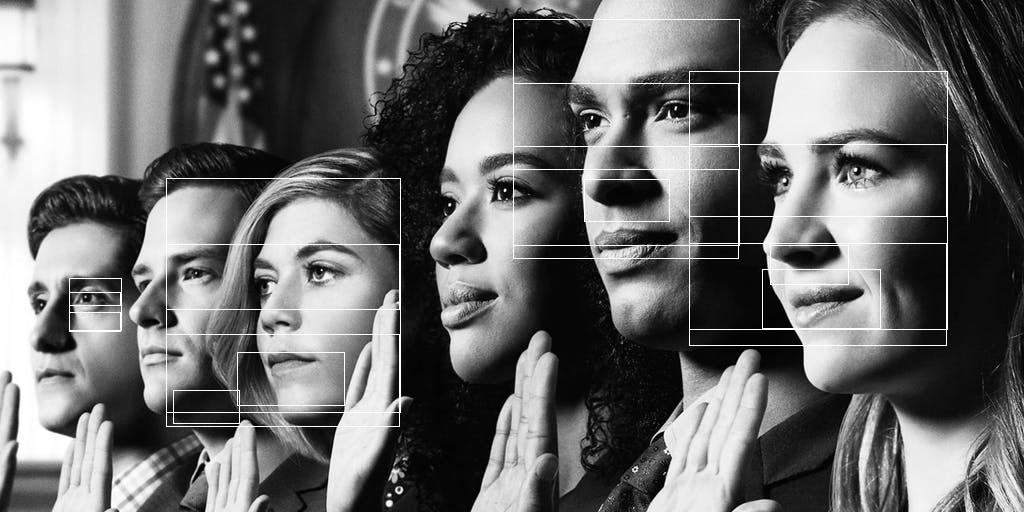
\includegraphics[scale = 0.4]{Face_track2.jpg}
		\caption{Múltiplas faces em uma imagem.}
	\end{figure}
	\newpage
	\section{Experimentos}
	\subsection{Aplicação da técnica em uma imagem de vídeo}
	Inicialmente, a técnica de reconhecimento foi aplicada em uma imagem de vídeo obtida através de uma câmera de computador onde ela procura catalogar e reconhecer vários elementos além do rosto da pessoa (no caso, os dois olhos e a boca), para melhor representação do método.
	\begin{figure}
		\centering
		\includegraphics[scale = 0.3]{ts5.png}
		\caption{Os dois olhos foram detectados separadamente (em branco).}
	\end{figure}
	\newpage
	\subsection{detecção de faces em uma imagem}
	No segundo teste, o algoritmo de detecção foi aplicado em duas imagem em tons de cinza bem definidas, e da mesma maneira que foi executada na imagem de vídeo, a recognição foi realizada normalmente.\\
	Nas imagens acima, que estão em boas condições, foram processadas por um algorítimo não muito diferentes do algorítmo de vídeo, mas que também processou a imagem para encontrar todas as faces possíveis, tantoque ele não detectou todas as faces direito na imagem superior.
	\vspace{4mm}
	\begin{figure}
		\centering
		\includegraphics[scale = 0.4]{s2.jpg}
		\caption{Uma Imagem em perfeitas condições.}
	\end{figure}
	\vspace{4mm}
	
	\newpage
	\section{Teste Definitivo: Detecção de faces em uma imagem em baixa qualidade}
	Por último, e mais importante, o algoritmo foi utilizado em uma imagem que continha várias faces, e ao mesmo tempo, possuía diferentes graus de péssima qualidade de visualização. Mesmo assim, com a baixa qualidade da imagem, a partir de um certo grau limite de baixa resolução e de um tamanho da face mínimo, o algorítimo consegue encontrar as faces.\\
	
	Para realizar múltiplas detecções, foi utilizado um vetor que armazena cada face ou elemento de face detectadas pelo algoritmo (cada elemento de cada vez), onde uma vez detectado uma face, a mesma face não vai ser detectada novamente.
	\begin{figure}
		\centering
		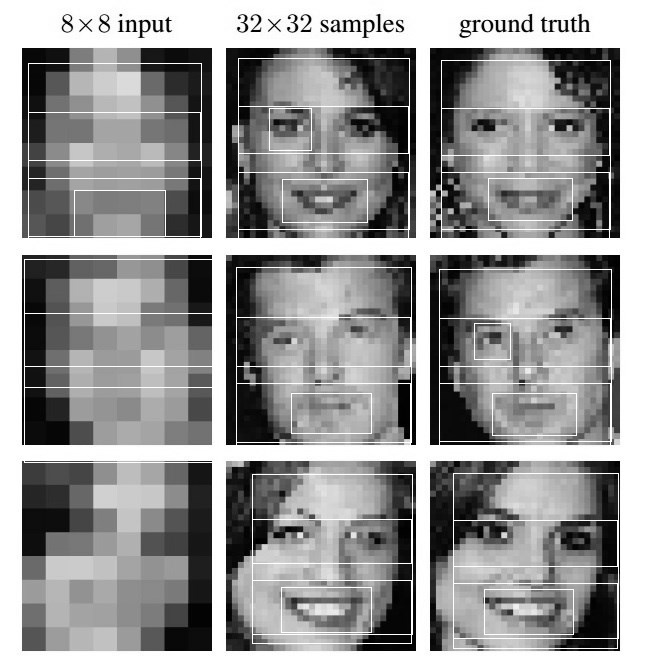
\includegraphics[scale = 0.4]{ft5.jpg}
		\caption{Imagem definitiva.}
	\end{figure}
	
	\newpage
	\section{Conclusão}
	Os códigos utilizados nesse trabalho, vide Apêndice, foram melhorados ou adaptados com o intuito de atender as exigências requeridas no mesmo. Os algorítmos utilizados para detectar as faces nas imagens foram adaptados para serem exibidos com maior visibilidade na detecção.
	\newpage
	\section{Apêndice}
	\subsection{Códigos do Trabalho}
	\subsubsection{facedetect modificado - ($facedetect\_mod.cpp$)}
	\begin{lstlisting}
#include "opencv2/objdetect/objdetect.hpp"
#include "opencv2/highgui/highgui.hpp"
#include "opencv2/imgproc/imgproc.hpp"

#include <iostream>
#include <stdio.h>

using namespace std;
using namespace cv;

void detectAndDraw( Mat& img);

CascadeClassifier cascadeFace, cascadeMouth;

String cascadeFaceName  = "haarcascade_frontalface_alt.xml";
String cascadeMouthName = "haarcascade_mcs_mouth.xml";

int main( int argc, const char** argv ){
CvCapture* capture = 0;
Mat frame, frameCopy, image;
VideoCapture cap(0);
int key;

if( !cascadeFace.load( cascadeFaceName )) {
cerr << "ERRO: Nao carregou filtro em cascata facefrontal" << endl;
return -1;
}
if( !cascadeMouth.load( cascadeMouthName )) {
cerr << "ERRO: Nao carregou filtro em cascata mouth" << endl;
return -1;
}

//  cap.set(CV_CAP_PROP_FRAME_WIDTH, 320);
//  cap.set(CV_CAP_PROP_FRAME_HEIGHT, 240);

for(;;){
cap >> frame;
flip(frame, frameCopy, 1); // inverte a imagem horizontalmente
///imshow("image", frameCopy);
//cout << "foi\n";
detectAndDraw(frameCopy); // detecta 

key = (char) waitKey(10);
if( key == 27 ) break;
}  
return 0;
}

void detectAndDraw( Mat& img){
int i = 0;
double t = 0;
vector<Rect> faces;

Mat gray;
cascadeFace.detectMultiScale(img, // imagem para deteccao
faces, // vetor com os retangulos encontrados
1.1, // escala de multiresolucao
3, // numero de vizinhos que cada candidato a retangulo
// devera contemplar. evita multiplas deteccoes parecidas
// na mesma regiao
0 | CV_HAAR_FIND_BIGGEST_OBJECT, // parametros (normalmente nao usados)
Size(30, 30) ); // minimo tamanho para deteccao de um objeto

for( vector<Rect>::const_iterator r = faces.begin(); r != faces.end(); r++ ){
Mat imgROI;
vector<Rect> nestedObjects;

rectangle(img,  
Point(r->x, r->y),  
Point(r->x + r->width, r->y + r->height),  
CV_RGB(255, 0, 0), 1, 8, 0);

if( cascadeMouth.empty() )
continue;

// posicao aproximada da boca em relacao a face...
Rect mouthROI = Rect(r->x, r->y + (r->height/1.5), 
r->width, r->height/2.5);    

rectangle(img, mouthROI, CV_RGB(255, 255, 0), 1, 8, 0);

imgROI = img(mouthROI);

cascadeMouth.detectMultiScale(
imgROI,
nestedObjects,
1.1,
2,
0 | CV_HAAR_FIND_BIGGEST_OBJECT,
Size(30, 30) );
// busca as bocas encontradas e desenha os retangulos
for( vector<Rect>::const_iterator nr = nestedObjects.begin(); nr != nestedObjects.end(); nr++ ){
rectangle(img,  
Point(r->x + nr->x, r->y + (r->height/1.5) + nr->y  ),  
Point(r->x + nr->x + nr->width, r->y + (r->height/1.5) + nr->y + nr->height),  
CV_RGB(255, 0, 255), 1, 8, 0);
}
}
imshow("Face track", img );
}
	\end{lstlisting}

	
	\newpage
	\subsubsection{face01 - ($face01.cpp$)}
	\begin{lstlisting}
#include "opencv2/objdetect/objdetect.hpp"
#include "opencv2/highgui/highgui.hpp"
#include "opencv2/imgproc/imgproc.hpp"

#include <iostream>
#include <stdio.h>

using namespace std;
using namespace cv;

void detectAndDraw( Mat& img);

CascadeClassifier cascadeFace, cascadeMouth, cascadeEye;

String cascadeFaceName  = "haarcascade_frontalface_alt.xml";
String cascadeMouthName = "haarcascade_smile.xml";
String cascadeEyeName = "haarcascade_eye_tree_eyeglasses.xml";

int main( int argc, const char** argv ){
//CvCapture* capture = 0;
Mat image;
//VideoCapture cap(0);
int key;

if( !cascadeFace.load( cascadeFaceName )) {
cerr << "ERRO: Nao carregou filtro em cascata facefrontal" << endl;
return -1;
}
if( !cascadeMouth.load( cascadeMouthName )) {
cerr << "ERRO: Nao carregou filtro em cascata mouth" << endl;
return -1;
}
if( !cascadeEye.load( cascadeEyeName )) {
cerr << "ERRO: Nao carregou filtro em cascata olho" << endl;
return -1;
}

//  cap.set(CV_CAP_PROP_FRAME_WIDTH, 320);
//  cap.set(CV_CAP_PROP_FRAME_HEIGHT, 240);

for(;;){
//cap >> frame;
//flip(frame, frameCopy, 1); // inverte a imagem horizontalmente
///imshow("image", frameCopy);
//cout << "foi\n";
image = imread(argv[1],CV_LOAD_IMAGE_GRAYSCALE);
detectAndDraw(image); // detecta 

key = (char) waitKey(10);
if( key == 27 ) break;
}  
return 0;
}

void detectAndDraw( Mat& img){
int i = 0;
double t = 0;
vector<Rect> faces;

Mat gray;
cascadeFace.detectMultiScale(img, // imagem para deteccao
faces, // vetor com os retangulos encontrados
1.1, // escala de multiresolucao
3, // numero de vizinhos que cada candidato a retangulo
// devera contemplar. evita multiplas deteccoes parecidas
// na mesma regiao
0 | CV_HAAR_FIND_BIGGEST_OBJECT, // parametros (normalmente nao usados)
Size(30, 30) ); // minimo tamanho para deteccao de um objeto

for( vector<Rect>::const_iterator r = faces.begin(); r != faces.end(); r++ ){
Mat imgROI, imgROI2;
vector<Rect> nestedObjects, nestedObjects2;

rectangle(img,  
Point(r->x, r->y),  
Point(r->x + r->width, r->y + r->height),  
CV_RGB(255, 255, 255), 1, 8, 0);

if( cascadeMouth.empty() )
continue;

// posicao aproximada da boca em relacao a face...
Rect mouthROI = Rect(r->x, r->y + (r->height/1.5), 
r->width, r->height/2.5);


rectangle(img, mouthROI, CV_RGB(255, 255, 255), 1, 8, 0);

imgROI = img(mouthROI);

cascadeMouth.detectMultiScale(
imgROI,
nestedObjects,
1.1,
2,
0 | CV_HAAR_FIND_BIGGEST_OBJECT,
Size(30, 30) );

// busca os olhos e as bocas encontradas e desenha os retangulos
for( vector<Rect>::const_iterator nr = nestedObjects.begin(); nr != nestedObjects.end(); nr++ ){
rectangle(img,  
Point(r->x + nr->x, r->y + (r->height/1.5) + nr->y  ),  
Point(r->x + nr->x + nr->width, r->y + (r->height/1.5) + nr->y + nr->height),  
CV_RGB(255, 255, 255), 1, 8, 0);
}
if( cascadeEye.empty() )
continue;
Rect eyeROI = Rect(r->x, r->y + (r->height/3.5), 
r->width, r->height/3.5);
rectangle(img, eyeROI, CV_RGB(255, 255, 255), 1, 8, 0);

imgROI2 = img(eyeROI);
cascadeEye.detectMultiScale(
imgROI2,
nestedObjects,
1.1,
2,
0 | CV_HAAR_FIND_BIGGEST_OBJECT,
Size(30, 30) );
for( vector<Rect>::const_iterator nr = nestedObjects.begin(); nr != nestedObjects.end(); nr++ ){
rectangle(img,  
Point(r->x + nr->x, r->y + (r->height/3.5) + nr->y  ),  
Point(r->x + nr->x + nr->width, r->y + (r->height/3.5) + nr->y + nr->height),  
CV_RGB(255, 255, 255), 1, 8, 0);
}
}
imwrite("Face_track.jpg", img );
imshow("Face track", img );
}
	\end{lstlisting}	
\end{document}